\subsection{Math problem-solving: partially-relational sequence-to-sequence tasks}\label{ssec:experiments_math}

The object-sorting experiments in the previous section are ``fully relational'' in the sense that the set of pairwise $\prec$ relations is a sufficient statistic for solving the task (i.e., the target sequence is conditionally independent of the input sequence given the relations). In general, in a generative sequence-to-sequence task, there may not be a relation which is a sufficient statistic. Nonetheless, relational reasoning may still be crucial for solving the task, and the enhanced relational reasoning capabilities of the Abstractor may enable performance improvements. The ``sensory-connected'' architectures described in~\Cref{sec:abstractor_architectures} enable a branch of the model to focus on relational reasoning while maintaining a connection to the sensory information of individual objects. In this section, we compare sensory-connected Abstractor models to standard Transformers on a set of math problem-solving tasks based on the dataset proposed in~\citep{saxtonAnalyzingMathematicalReasoning2019}.

The dataset consists of several math problem-solving tasks, with each task having a dataset of question-answer pairs. The tasks include solving equations, expanding products of polynomials, simplifying polynomials, differentiating functions, predicting the next term in a sequence, etc. A sample of question-answer pairs are displayed in~\Cref{fig:math_dataset}.

% TODO: create this figure
\begin{figure}
    \begin{minipage}{0.5\textwidth}
        % \centering
        Task: \texttt{polynomials\_\_expand}\\
        Question: \texttt{Expand (2*x + 3)*(x - 1).}\\
        Answer: \texttt{2*x**2 + x - 3}\\

        Task: \texttt{algebra\_\_linear\_1d}\\
        Question: \texttt{Solve for z: 5*z + 2 = 9.}\\
        Answer: \texttt{7/5}\\
    \end{minipage}
    \caption{Examples of input/target sequences from the math problem-solving dataset.}\label{fig:math_dataset}
\end{figure}


\begin{table}[p]
    \begin{tabular}{llrr}
\toprule
                    &                            &  tf acc &  tf acc (val) \\
task & model &         &               \\
\midrule
algebra\_\_linear\_1d & transformer &   0.706 &         0.661 \\
                    & transformer+ &   0.664 &         0.612 \\
                    & relational\_abstractor &   0.814 &         0.759 \\
                    & relational\_abstractor (v2) &   0.714 &         0.607 \\\hline
algebra\_\_sequence\_next\_term & transformer &   0.831 &         0.865 \\
                    & transformer+ &   0.833 &         0.864 \\
                    & relational\_abstractor &   0.885 &         0.910 \\
                    & relational\_abstractor (v2) &   0.866 &         0.901 \\\hline
calculus\_\_differentiate & transformer &   0.969 &         0.991 \\
                    & transformer+ &   0.981 &         0.995 \\
                    & relational\_abstractor &   0.990 &         0.997 \\
                    & relational\_abstractor (v2) &   0.986 &         0.996 \\\hline
comparison\_\_kth\_biggest & transformer &   0.894 &         0.898 \\
                    & transformer+ &     NaN &           NaN \\
                    & relational\_abstractor &   0.991 &         0.993 \\
                    & relational\_abstractor (v2) &   0.984 &         0.988 \\\hline
comparison\_\_sort & transformer &   0.995 &         0.998 \\
                    & transformer+ &     NaN &           NaN \\
                    & relational\_abstractor &   0.997 &         0.999 \\
                    & relational\_abstractor (v2) &   0.997 &         0.988 \\\hline
polynomials\_\_add & transformer &   0.838 &         0.833 \\
                    & transformer+ &   0.846 &         0.843 \\
                    & relational\_abstractor &   0.858 &         0.857 \\
                    & relational\_abstractor (v2) &   0.857 &         0.857 \\\hline
polynomials\_\_coefficient\_named & transformer &   0.565 &         0.537 \\
                    & transformer+ &   0.562 &         0.533 \\
                    & relational\_abstractor &   0.587 &         0.557 \\
                    & relational\_abstractor (v2) &   0.575 &         0.547 \\\hline
polynomials\_\_collect & transformer &   0.898 &         0.892 \\
                    & transformer+ &     NaN &           NaN \\
                    & relational\_abstractor &   0.949 &         0.950 \\
                    & relational\_abstractor (v2) &   0.934 &         0.929 \\\hline
polynomials\_\_compose & transformer &   0.805 &         0.794 \\
                    & transformer+ &     NaN &           NaN \\
                    & relational\_abstractor &   0.837 &         0.825 \\
                    & relational\_abstractor (v2) &   0.835 &         0.824 \\\hline
polynomials\_\_evaluate & transformer &   0.652 &         0.593 \\
                    & transformer+ &     NaN &           NaN \\
                    & relational\_abstractor &   0.697 &         0.615 \\
                    & relational\_abstractor (v2) &   0.708 &         0.634 \\\hline
polynomials\_\_expand & transformer &   0.777 &         0.757 \\
                    & transformer+ &   0.778 &         0.758 \\
                    & relational\_abstractor &   0.814 &         0.795 \\
                    & relational\_abstractor (v2) &   0.794 &         0.775 \\
\bottomrule
\end{tabular}

    \caption{Metrics for the math problem-solving tasks.}\label{tab:math_metrics}
\end{table}

\begin{table}[p]
    \begin{tabular}{llrr}
\toprule
                    &                       &  tf acc &  tf acc (val) \\
task & model &         &               \\
\midrule
algebra\_\_linear\_1d & transformer &   0.792 &         0.733 \\
                    & transformer+ &   0.776 &         0.603 \\
                    & relational\_abstractor &   0.834 &         0.791 \\
algebra\_\_sequence\_next\_term & transformer &   0.889 &         0.881 \\
                    & transformer+ &   0.922 &         0.918 \\
                    & relational\_abstractor &   0.916 &         0.922 \\
calculus\_\_differentiate & transformer &   0.996 &         0.998 \\
                    & transformer+ &   0.998 &         0.998 \\
                    & relational\_abstractor &   0.999 &         1.000 \\
polynomials\_\_add & transformer &   0.851 &         0.841 \\
                    & transformer+ &   0.860 &         0.851 \\
                    & relational\_abstractor &   0.869 &         0.863 \\
polynomials\_\_coefficient\_named & transformer &   0.587 &         0.549 \\
                    & transformer+ &   0.603 &         0.564 \\
                    & relational\_abstractor &   0.630 &         0.599 \\
polynomials\_\_expand & transformer &   0.804 &         0.774 \\
                    & transformer+ &   0.817 &         0.785 \\
                    & relational\_abstractor &   0.847 &         0.821 \\
\bottomrule
\end{tabular}

    \caption{Metrics for the math problem-solving tasks (tfm implementation).}\label{tab:math_tfm_metrics}
\end{table}

\begin{figure}
    \centering
    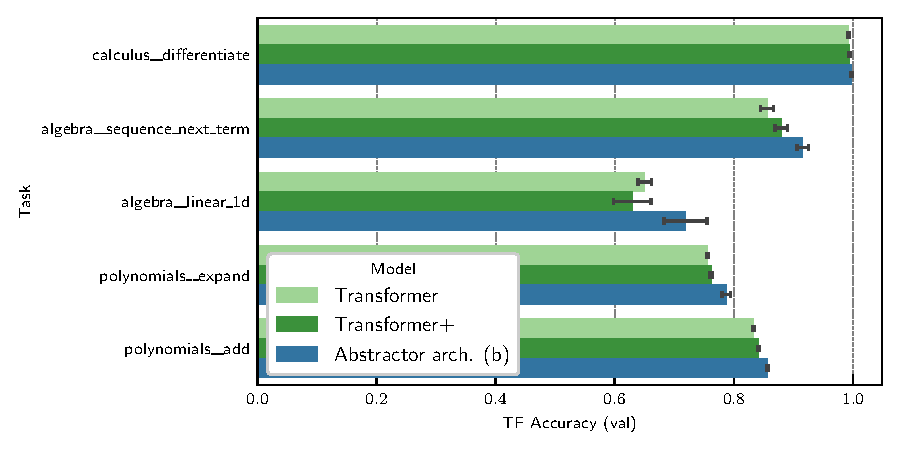
\includegraphics{figures/experiments/math_metrics.pdf}
    \caption{`from scratch' implementation}\label{fig:math_metrics}
\end{figure}

\begin{figure}
    \centering
    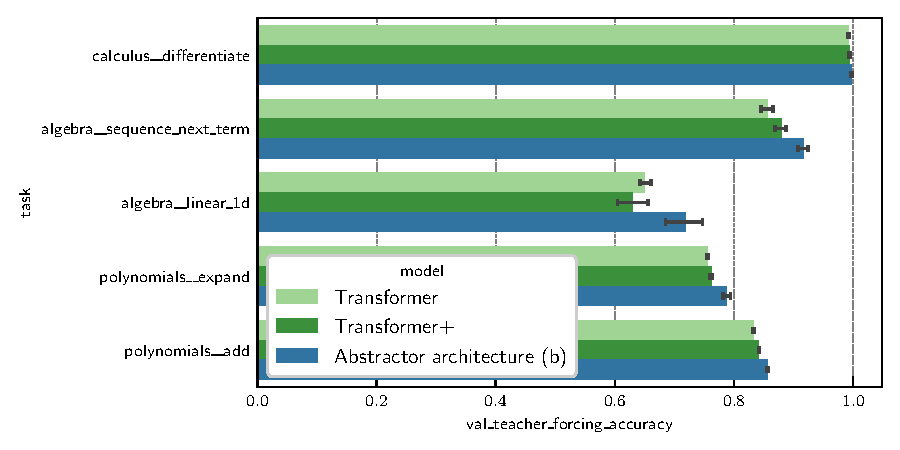
\includegraphics{figures/experiments/math_tfm_metrics.pdf}
    \caption{tfm implementation}\label{fig:tfm_math_metrics}
\end{figure}